\section{Exercise 4 - Binary Tree Algorithms for \texttt{MPI\_Bcast} and \texttt{MPI\_Reduce}}

Instead of “lined up” processes we now want to use a binary tree structure and according algorithms 
\texttt{MY\_Reduce\_T()} and \texttt{MY\_Bcast\_T()} for reduction and broadcasting. As we understand 
each process as a node, we will use the wording node from now on. For indexing of the nodes, we use preorder traversal.

\begin{figure}[h]
    \begin{center}
        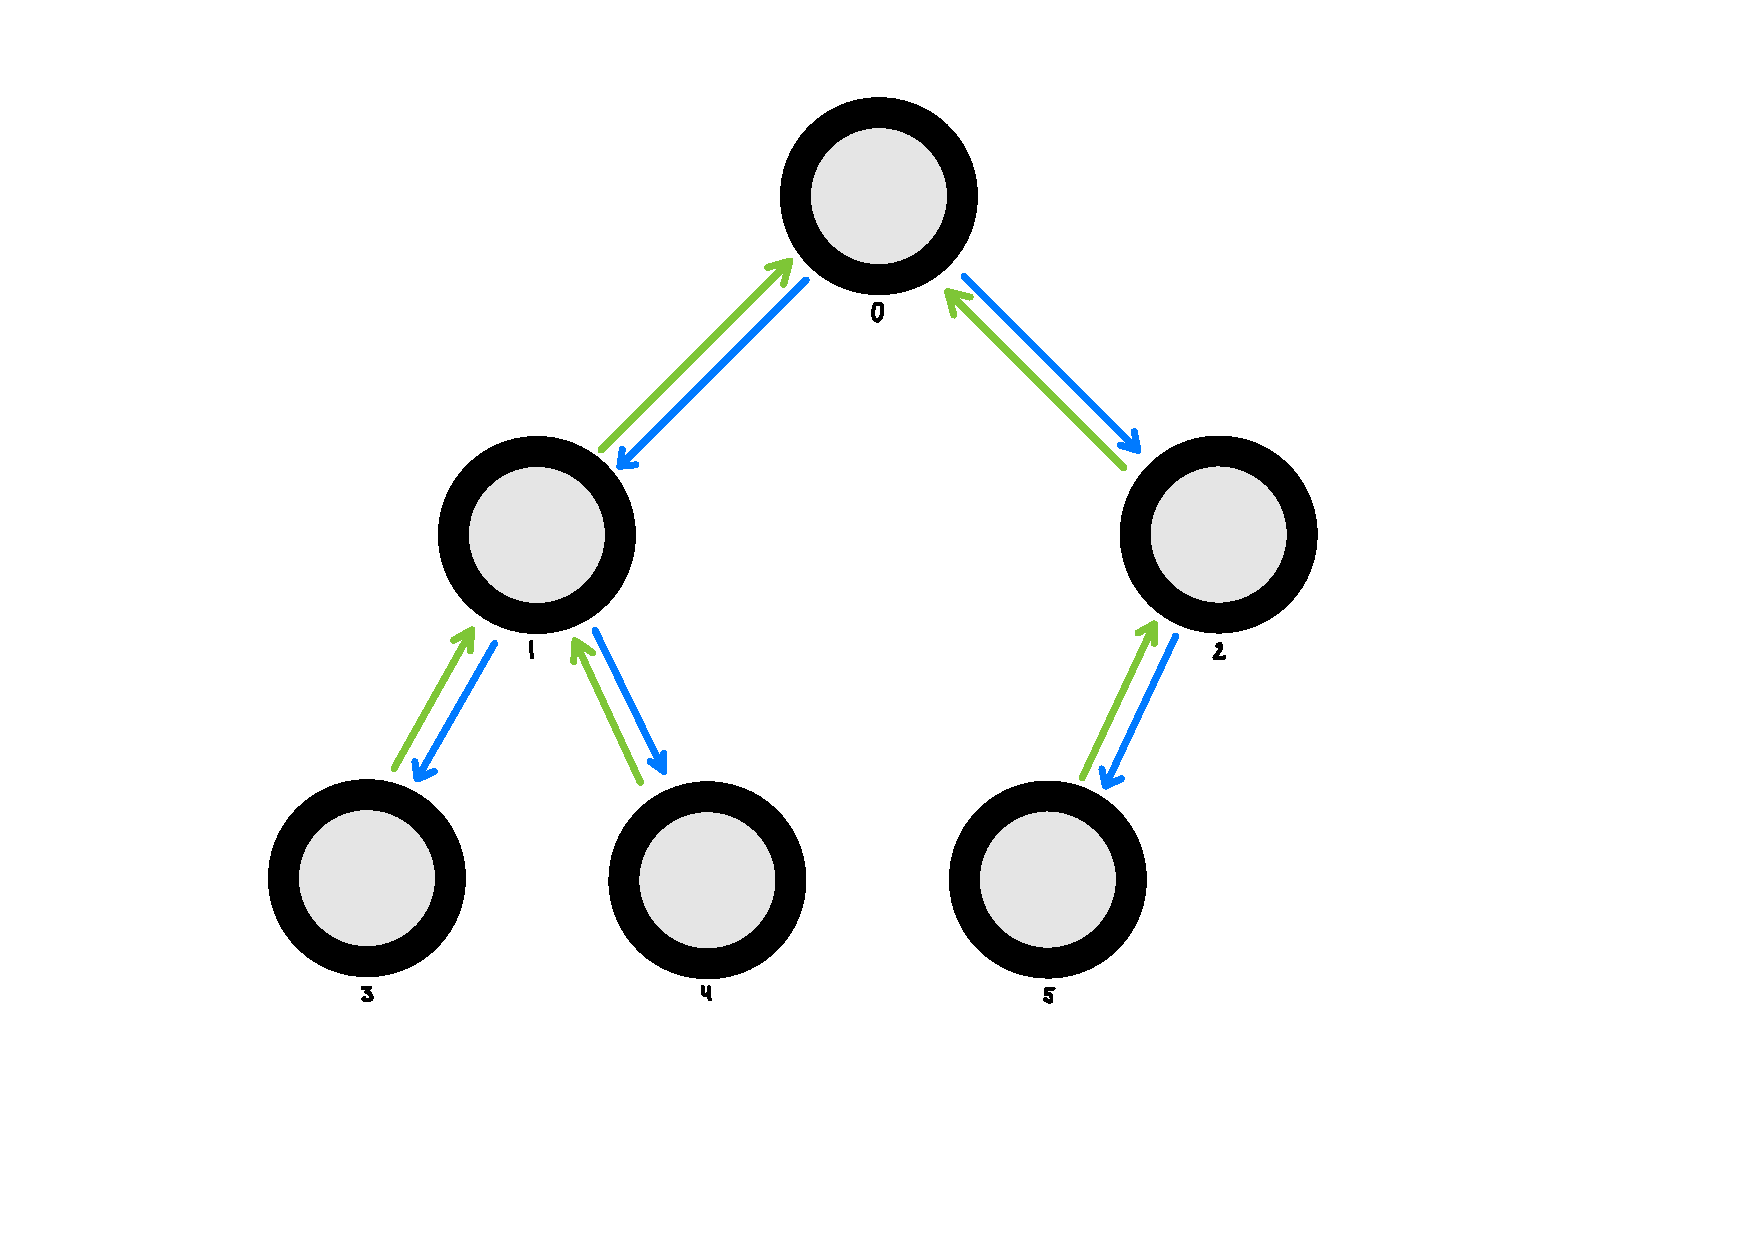
\includegraphics[width=0.6\linewidth]{figures/sketch_tree.pdf}
        \caption{Binary tree topology for message passing scheme in exercises 4 and 5}
        \label{Ex4_sketch_p}
    \end{center}
\end{figure}

We start very similar to the implementations of \texttt{MY\_Reduce\_P()} and \texttt{MY\_Bcast\_P()} 
from exercise 2. For the reduction \texttt{MY\_Reduce\_P()}  the root node (rank $=0$) on level 0 should 
gain the reduced result. Hence, the leaves start by sending the data block by block to their parents. All 
interior nodes receive exactly two data blocks per communication round. One from their left and one from their 
right child. After performing a local reduction, the data is sent to the nodes parent. In the end, the root 
node receives the data from its two children and ends up with the reduction result. For the broadcast 
\texttt{MY\_Bcast\_P()}, the root node sends the data block wise to its two children. A child receives 
the data and immediately forwards this data to its children, in case it is not a leaf.\\

The trivial combination of \texttt{MY\_Reduce\_T()} and \texttt{MY\_Bcast\_T()} can be seen 
as a pipelined variant of \texttt{MPI\_Allreduce()}.\\

For performance estimation -- again -- let us consider the number of communication rounds between processes in the 
just discussed implementatations of \texttt{MY\_Reduce\_T()} and \texttt{MY\_Bcast\_T()}. In figure 
\ref{Ex4_sketch_p} the considered binary tree structure can be seen ver well. The green arrows 
indicate the communication steps for \texttt{MY\_Reduce\_T()} and the blue arrows \texttt{MY\_Bcast\_T()}. 
Only once all reduction communications are finished (green arrows), the broadcasting (blue) starts -- same as discussed in 
exercise 2. 

\pagebreak

The path of the exercise 4 graph after count = $10^3$ would normally continue to intercept and perfrom worse
than the others plotted, due to the blocksize adjustment that occurs at count = $10^6$ this does not happen.

\begin{figure}[h]
    \begin{center}
        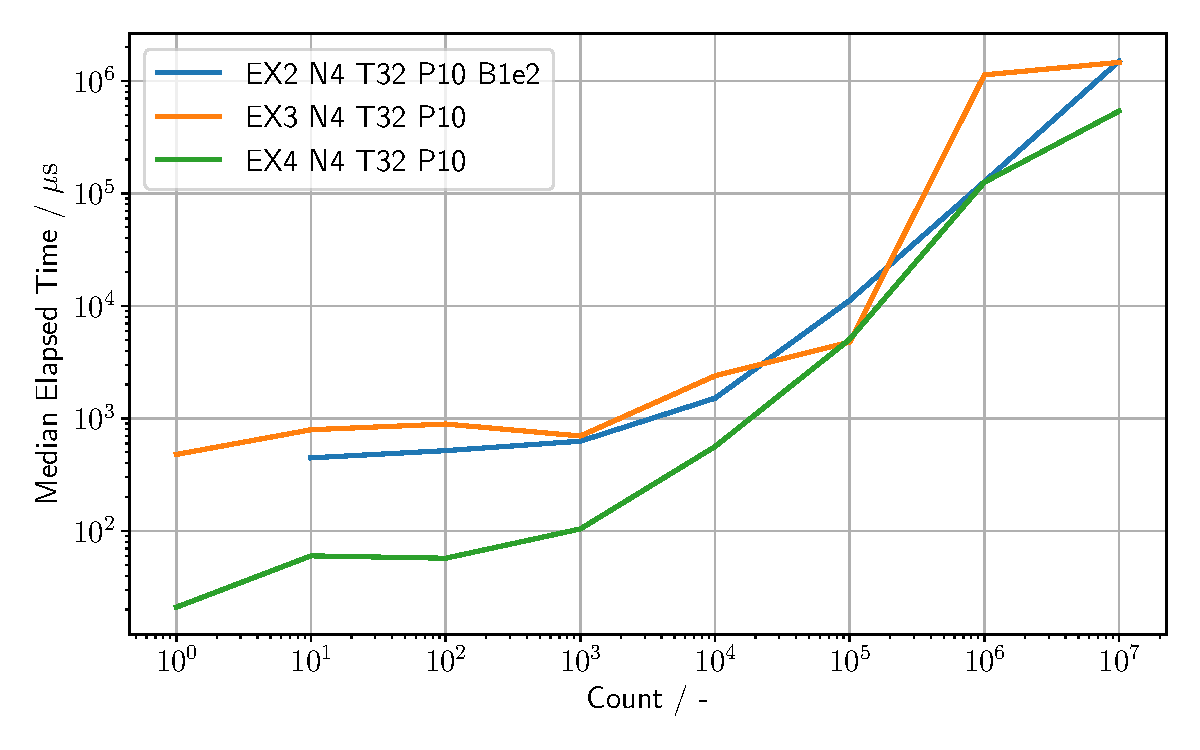
\includegraphics[width=0.85\linewidth]{figures/Ex4_1.pdf}
        \caption{Median elapsed time for 4 nodes, 32 tasks per node and powers of 10. Clearly visible improvement
        over all count sizes. At count = $10^5$ the \fun{MY\_Allreduce\_P()} outperforms the tree algorithm
        \fun{MY\_Reduce\_T()} + \fun{MY\_Bcast\_T()} slightly. At count = $10^6$ the tree algorihtm and the 
        blocksize = 100 algorithm from exercise 2 coincide.}
        \label{Ex4_1_p}
    \end{center}
\end{figure}

In figures \ref{Ex4_3_p} and \ref{Ex4_4_p} below, we can observe the slope improvements again due to the
blocksize adjustment. What also pops out is that the graphs are tightly packed and appear to perform similar
even though they have different configurations regarding the tasks per node. 

\begin{figure}[h]
    \centering
        \begin{minipage}[t]{.49\textwidth}
            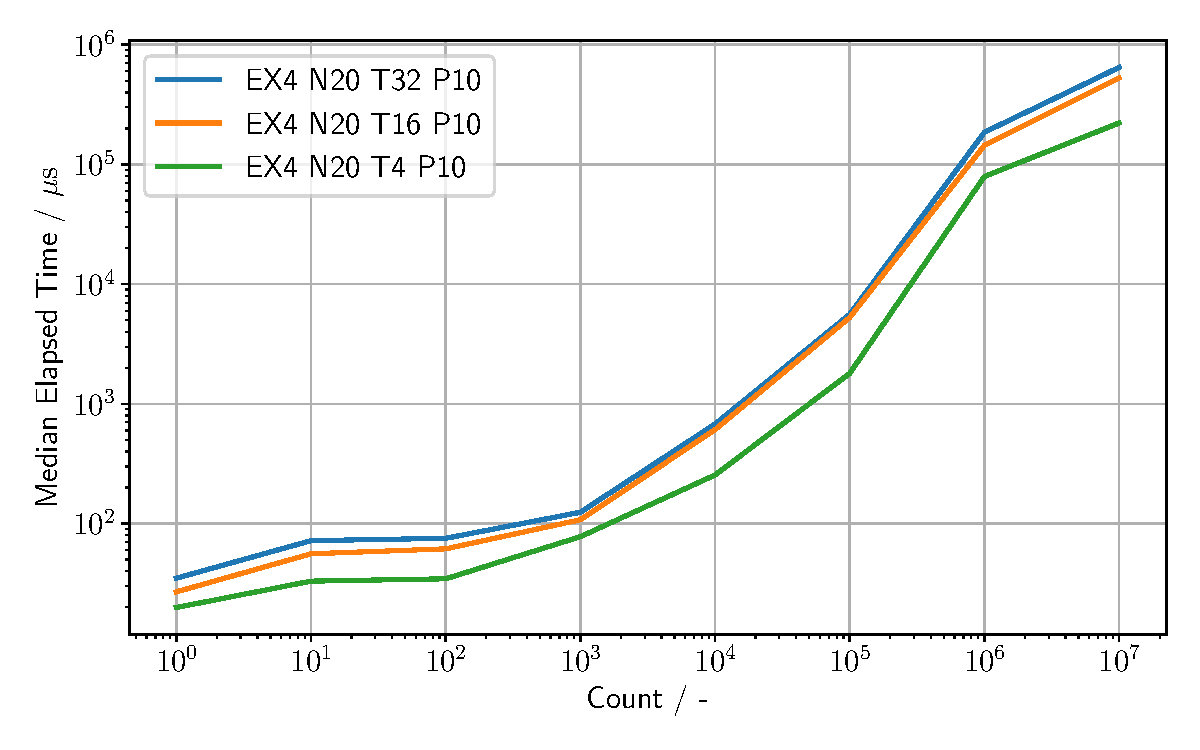
\includegraphics[width=1\linewidth]{figures/Ex4_3.pdf}
            \captionof{figure}{\fun{MY\_Reduce\_T()} + \fun{MY\_Bcast\_T()} tree algorithm with 20 
            nodes and powers of 10. Visible slope reduction due to blocksize adjustment 
            at count = $10^6$ again.}

            \label{Ex4_3_p}
        \end{minipage}
        \hfill
        \begin{minipage}[t]{.49\textwidth}

            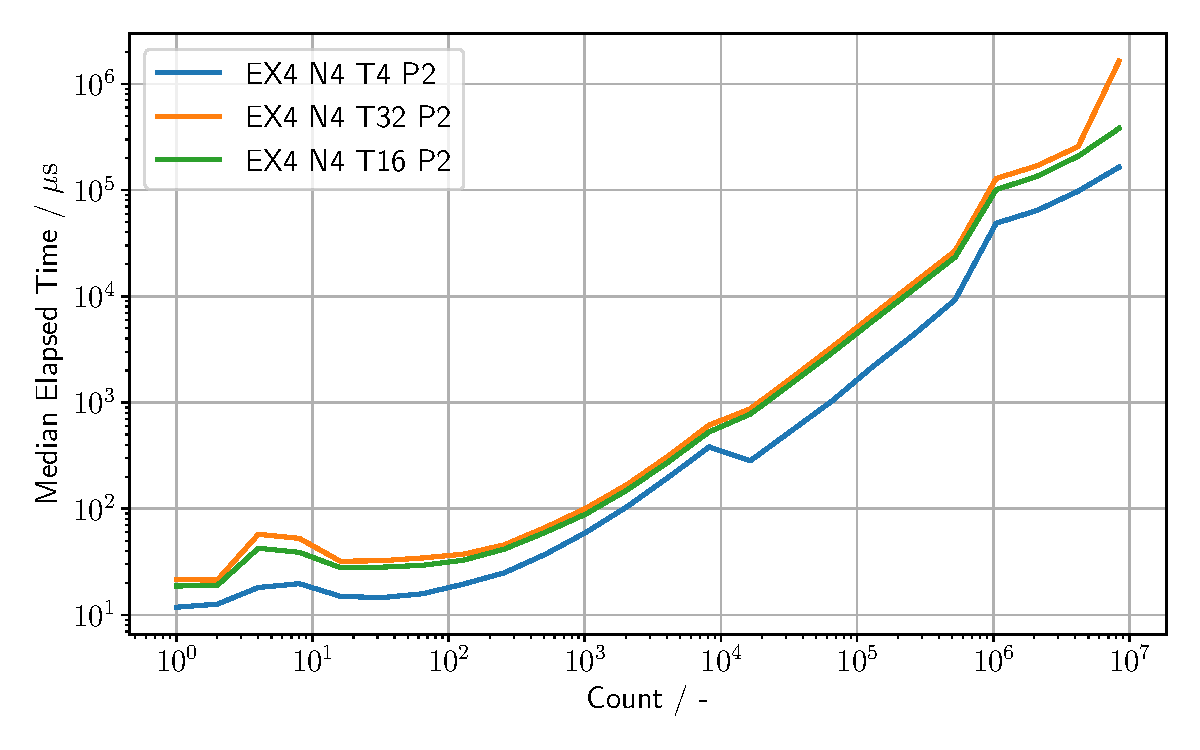
\includegraphics[width=1\linewidth]{figures/Ex4_4.pdf}
            \captionof{figure}{\fun{MY\_Reduce\_T()} + \fun{MY\_Bcast\_T()} tree algorithm with 20 
            nodes and powers of 2. Visible slope reduction due to blocksize adjustment 
            at count = $10^6$ as well.}

            \label{Ex4_4_p}
        \end{minipage}
    \end{figure}

\pagebreak